\chapter{Flujos de trabajo sobre cómputo en la nube}

En este capítulo, describiremos el algoritmo que es la pieza clave del sistema para agendar tareas de un flujo de trabajo en infraestructura de cómputo en la nube, tomando en cuenta los lineamientos de diseño propuestos anteriormente.



\section{Antecedentes}

También, un área de investigación activa es la planificación de tareas a nivel de procesador (CPU's), en donde se asume que se tiene un procesador cuyos núcleos son idénticos e intercambiables. Además, en los trabajos de investigación referentes a esta área se consideran a los grafos dirigidos acíclicos como los modelos de tareas más generales. Así, basados en el trabajo de Saifullah et al. \cite{saifullah2013multi}, en donde primero se transforma un grafo dirigido acíclico en un conjunto de tareas secuenciales con secciones que se ejecutan en paralelo.


% Podemos hacer esto aún más abstracto y combinarlo con la teoría de Pinedo

% EFT: Earliest-Finish Time
% DM: Deadline Monotonic
% EDF: Earliest-Deadline First
% Global EDF
% Partitioned EDF

% how to enable theory with processor teory
% I think my thesis is that weird link, with the basic paper
% no hay que olvidar que hay que optimizar tiempo, dinero

% ya sabemos que es NP-hard, asi que nos enfocaremos en el problema



% Primero, tienes recursos 'infinitos', solo sujetos a presupuesto
% puedes averiguar el numero maximo de maquinas a levantar con el modelo de tareas paralelar
% simplemente cuentas el segmento con el mayor numero de paralelizaciones

Es muy común que los servicios de cómputo en la nube se paguen la utilización de las máquinas virtuales por hora, dejando sin cobrar porciones de hora no utlizadas. Además, se pueden solicitar tantos recursos como se requieran, limitándose solamente al presupuesto disponible. Además, estas máquinas virtuales son recursos variados; pueden ser desde máquinas con un solo procesador, hasta VM's con grandes cantidades de memoria.

De acuerdo al primer capitulo del libro de Pinedo \cite{pinedo2012scheduling} hay esfuerzos para clasificar los problemas de planificación en general. Sin embargo, la clasificación presentada en este trabajo sólo contempla los problemas que optimizan una sola métrica. Aunque, se puede utilizar una combinación lineal de funciones objetivo a optimizar y de esta forma se pueden utilizar estos algoritmos de planificación. Sin embargo, esta forma de atacar el problema de planificación multiobjetivo no garantiza evaluar todas las posibles opciones. 

% Hacer puente entre las teorías de Buyya y Jia Yu y las teorías de Pinedo

% Hay que leer los papers de arquitectura



\section{Los cuatro algoritmos}

Si bien en la literatura hay múltiples algoritmos de planificación publicados por la comunidad científica, éste es sólo una parte (muy importante) de un sistema administrador de flujos de trabajo. En el caso de este trabajo, dividmos todo el proceso en cuatro fases:

\begin{enumerate}
\item{Planificación}
\item{Asignación de recursos}
\item{Ejecución}
\item{Descarga de resultados}
\end{enumerate}



\subsection{Planificación}

La idea base del algoritmo es lidiar con las dependencias, ya que éstas generan restricciones sobre el problema. Otra característica a aprovechar es el hecho de que los recursos de cómputo en la nube pueden ser tratados como \emph{efímeros}, es decir, pueden ser creados y destruidos conforme se vayan necesitando.

De esta forma, el primer paso del algoritmo de planificación es dividir el flujo de trabajo en segmentos consecutivos, con la propiedad de que un segmento sólo dependa de la ejecución completa del segmento anterior

Para generar los segmentos, se utiliza la definición de Saifullah et. al \cite{saifullah2013multi} basada en la profundidad de cada nodo del DAG que representa el flujo de trabajo.

\begin{defn}

La \textbf{profundidad} $h$ de una tarea $t$ de un flujo de trabajo está definida como:

\begin{displaymath}
h(x) = \left\{
     \begin{array}{lr}
       \max_{u \in \text{Padres}(t) } h(u) + 1 & : | \text{Padres}(t) | \neq 0 \\
       1                                       & : | \text{Padres}(t) | = 0
     \end{array}
   \right.
\end{displaymath}

\noindent Donde $\text{Padres}(t)$ es el conjunto de tareas que inmediatamente preceden a la tarea $t$, es decir, aquellas tareas $u$ que tienen una dependencia de orden que va a la tarea $t$.
\end{defn}

En la figura \ref{fig:DAG_to_segment} se puede apreciar un ejemplo de este algoritmo, en donde se puede ver que a cada tarea del flujo de trabajo se le asigna un segmento, en cual se está garantizando que cada segmento sólo dependa del segmento anterior.

\begin{figure}
\begin{center}
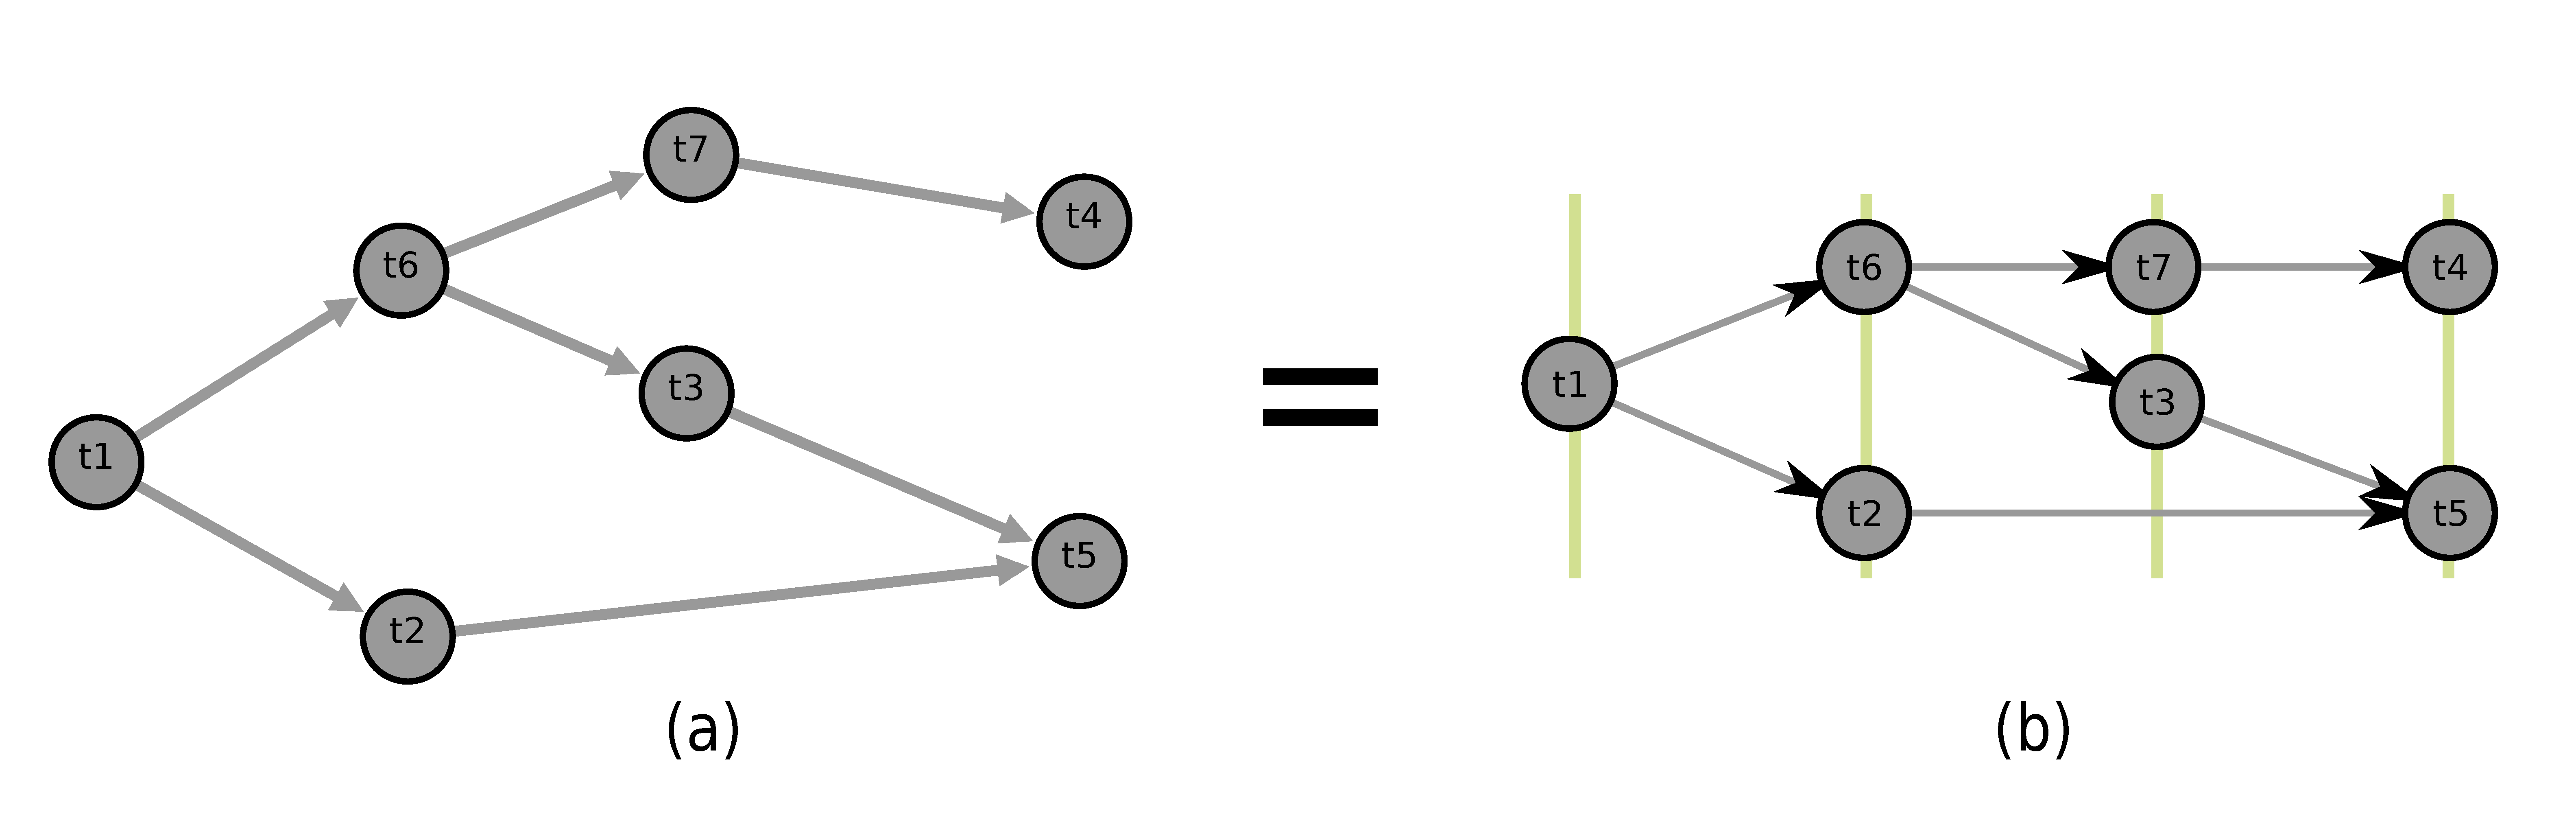
\includegraphics[width=1.0\textwidth]{imagenes/DAG_to_segment.pdf}
\end{center}
\caption{Transformación de un flujo de trabajo (a) a segmentos (b)}
\label{fig:DAG_to_segment}
\end{figure}

